\section{Estimate Speed}

To reveal the correlation of user's speed and mobile data access patterns, we first need to estimate a user's speed. We aimed to estimate a user's speed solely from the mobile access data traces without extra location information. The challenge lies in three aspects. First, such large-scale traces usually have very low accuracy of location estimation, in our dataset, the only location information is the coordinate of the towers with which the users communicate. So the location estimation error is the whole coverage area of towers, for towers located in suburban areas, the coverage of a single tower could have a diameter of several kilometers. Moreover, a user may not generate any mobile data traffic for a long time due to light usage of apps or the apps does not require network access. So the time interval between consecutive records could be very large and the towers they connected to could be far apart. We have little information of where the user was during these blank periods. In the last, even the tower that was recorded in the trace may not be accurate due to the fact that wireless communication range of a towers may fluctuate. Even a user did not move at all, he still might have communicated with more than one tower. 

\subsection{Structure overview}

\begin{figure*}[ht]
    \centering
    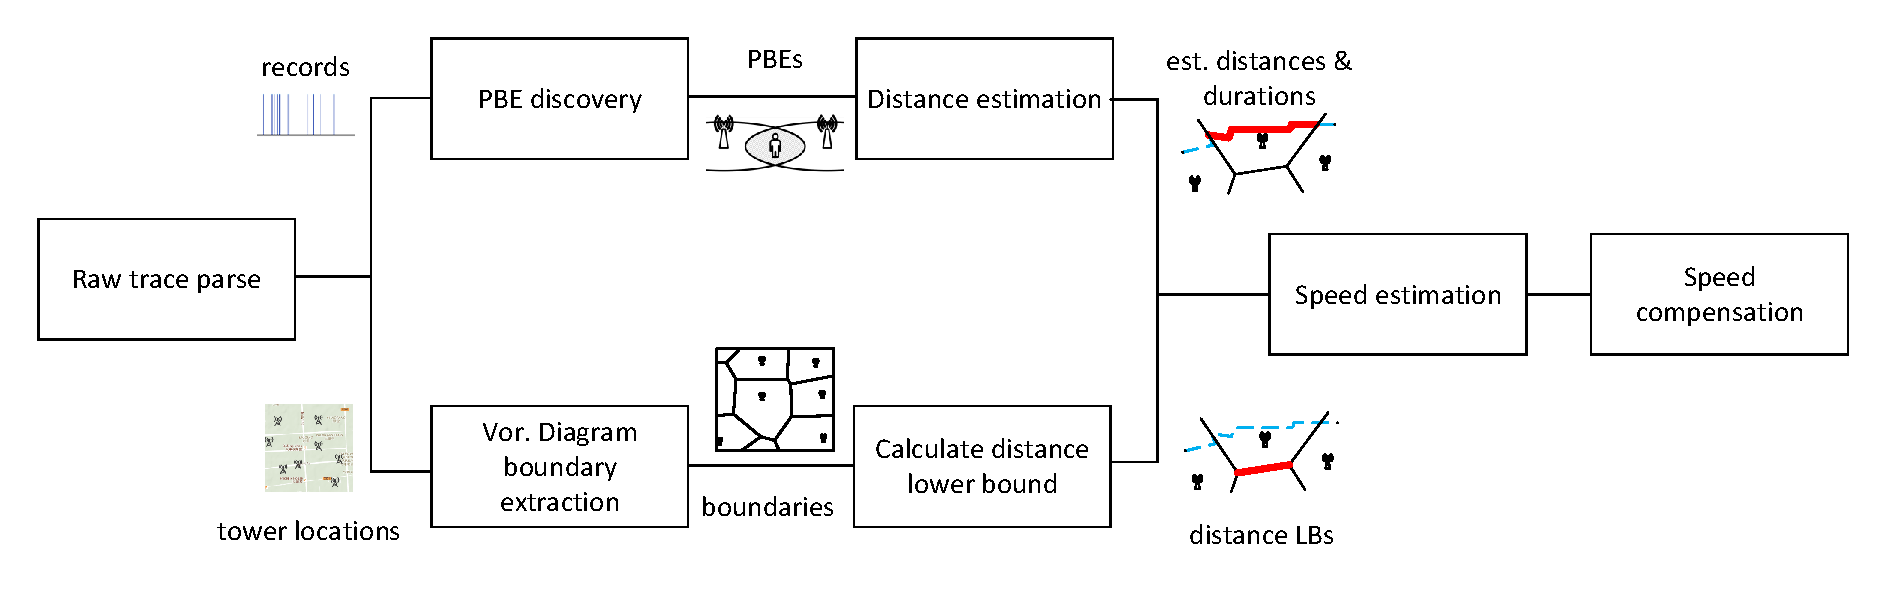
\includegraphics[width=\linewidth]{./figures/system_overview.pdf}
    \caption{Speed estimation system overview}
    \label{fig:system_overview}
\end{figure*}

Fig.~\ref{fig:system_overview} shows the structure overview of how we process our data. The raw data parser first gather data access records and tower locations from the mobile data access trace. Then the passing boundary events are extracted from the data access records. Based on these passing boundary events, traveled distances and durations are estimated. With tower locations, a Voronoi diagram is built and Voronoi ridges are collected to be used to approximate the communication coverage boundaries between towers. And distance lower bounds for each user to pass a tower's coverage area are estimated based on the approximated boundaries. With distance estimations, distance lower bounds and duration estimates, the system can estimate the user's speed and filter out inaccurate speed estimates with criterion based distance lower bounds and duration estimates. For some records that do not have sufficient location information to accurately estimate the user's speed, the system will also compensate their speed estimation. We will discuss each component in more details in the following sections.

\subsection{Passing boundary event}

\begin{figure}[h]
    \centering
    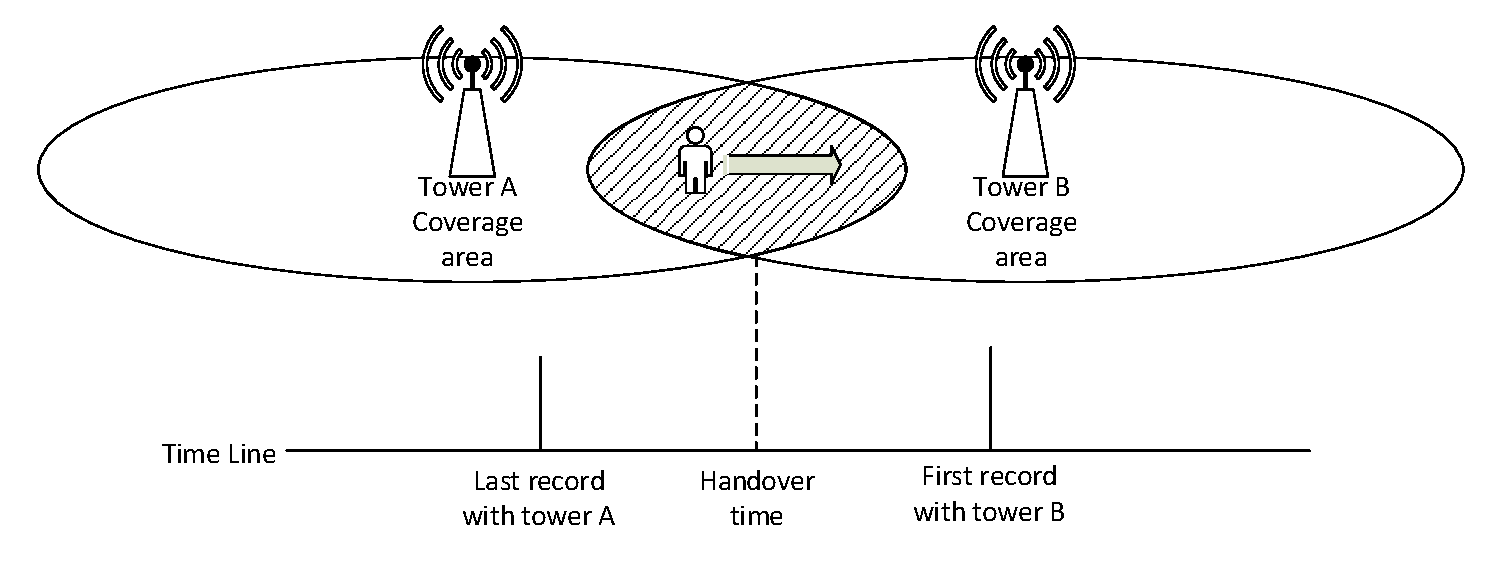
\includegraphics[width=\linewidth]{./figures/passing_boundary.pdf}
    \caption{Passing boundary event.}
    \label{fig:pass_bound}
\end{figure}

For arbitrary two consecutive records $r_i$ and $r_j$ from the sorted mobile data access records of a user, if they have different related tower location, we define them as a PBE (passing boundary event), denoted by $P_{i,j}$:
\[
P_{i,j} = (r_i, r_j),  where l_i \neq l_j
\]
For example, in fig.~\ref{fig:pass_bound}, a user moved from tower A's coverage area to tower B's coverage area. The switch from tower A to tower B should happen in the overlapped area which is shown with shadows. Although we don't know exactly when the switch happened, but the time should be bounded by the time of last record with tower A and the time of first record with tower B. So for a PBE, the time of the event is a time interval defined by the time of the two related records $(t_i, t_j)$. Note that since the mobile data access of a user are not continuous and user may communicate with towers that are far away from each other in two consecutive records. So for the boundary related to the event, if the two towers are adjacent with each other, i.e. their communication coverage overlap, then the boundary of the even is the overlapped boundary area and we refer to it as a real boundary. Otherwise, the boundary of the event is refer to as a virtual boundary. 

The reason for using PBE is that PBEs with real boundaries have better location estimation accuracy. The location estimation accuracy of an arbitrary record $r_i$ is the whole coverage area of the related tower $l_i$. For a PBE $P_{i,j}$ with a real boundary, the location accuracy of the boundary is the overlapped boundary area of the two related towers. Since the boundary area is only a sub-area of whole coverage areas of both towers. The location accuracy of PBE $P_{i,j}$ is better than location accuracy of both related records $r_i$ and $r_j$. By combining location information in two consecutive records that have different location estimates, we can achieve a better location estimation accuracy.

Note that the better location accuracy only stands for PBEs with real boundaries. Since there are no overlaps for two towers of a virtual boundary, it's hard to make any assumptions of the size of boundary area compared to the size of coverage area of related towers. The possible boundary area of a virtual boundary could be much larger than the coverage area of both towers. In some cases, it may including the communication areas of multiple towers. 

We rearrange our data by aggregating mobile data access records between two consecutive PBEs as a single unit called aggregate mobile data access record. All records belonging to the same aggregate record are communicate with the same tower. An aggregate mobile data access record is the minimum unit when we estimate the speed, that is, all records belonged to the same aggregate record will have the same speed estimate with our algorithm. The reason for this is that we don't have sufficient location information to differentiate records belonging to the same aggregate record. Each aggregate record has one (the first and the last session) or two PBEs related to it. Note that our algorithms can only estimate speed for aggregate record with two PBEs. So the first and last aggregate record will not have a speed estimation with only one PBE. This means users that have traveled less than three tower will not have speed estimate for any record at all. For example, in Fig.~\ref{fig:typical_user}, there are 6 aggregate record. Only from the second aggregate record to the fifth aggregate record have both PBEs. So we won't have speed estimate for the first aggregate record and the last (sixth) aggregate record. 

\subsubsection{travel distance estimation}

With the knowledge of location of visited towers and the sequence in which a user visited them, one can easily come up with a estimated trajectory based on the maximum likelihood of each possible trajectories and the sequence of visited towers. And an estimated travel distance can be easily calculated from the estimated trajectory. But the real cases is much more complicated that makes such approach not so accurate. One common problem in our and similar datasets is that, according to the data access records, users seem to pass some tower's coverage area in very short amount of time. For example in fig.~\ref{fig:typical_user}, the user passing through tower B and tower E's coverage area so quickly that if we use the distance estimates we acquire from such approaches, we will end up with unrealistic speed estimates. There are various reasons may cause these short passing through time problem. For example in fig.~\ref{fig:illustrate_cases}, solid lines represent real user trajectory while dashed lines represent boundaries of towers. In the left part we show a user's trajectory intersects with the boundary for a few time, in this case, the user is likely to keep switching between tower A and tower B. So the trace of the user will be cut into several mini sections, each with a quiet short period of time. Actually, when taking the communication range fluctuation problem into consideration, even when a user stay still near the boundaries, he is likely to produce several false passing boundary events. Another problem is shown in the right part of fig.~\ref{fig:illustrate_cases}. Even without the false passing boundary events, in this case, we can see that there are various paths with different distance to passing through tower B's coverage area. This means using a single distance estimate can never be accurate for such scenarios as it fails to adapt to various possible situations without additional location information.

\begin{figure}[h]
    \centering
    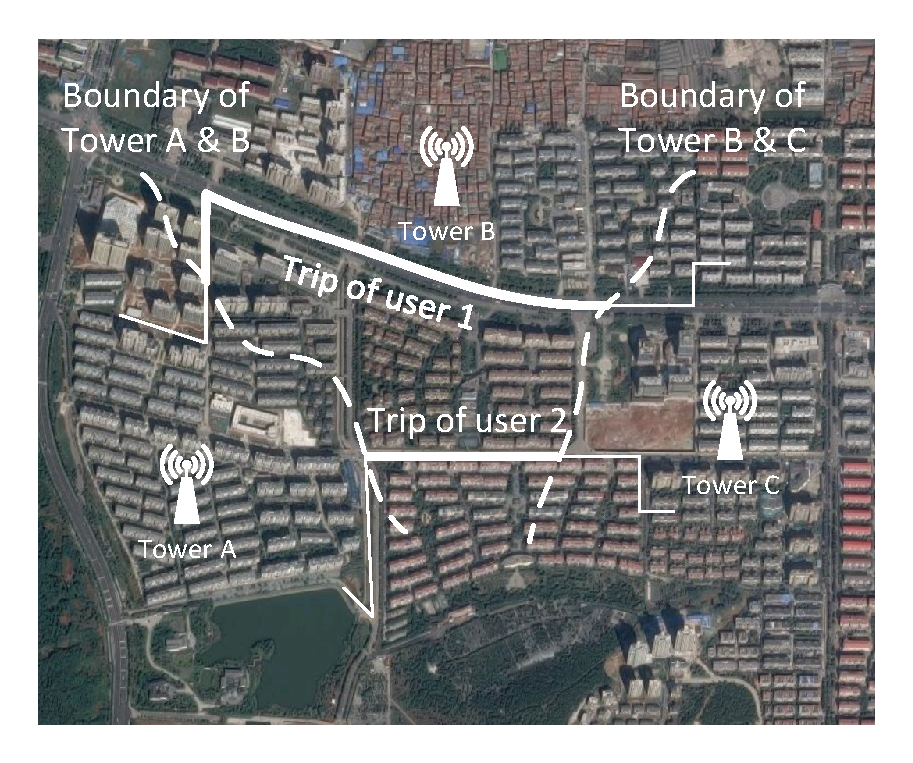
\includegraphics[width=\linewidth]{./figures/illustrate_cases.pdf}
    \caption{Common cases where a distance estimate will fail}
    \label{fig:illustrate_cases}
\end{figure}

To make our distance estiamtes more robust to cases shown in fig.~\ref{fig:illustrate_cases}, we not only need to calculate an estimated distance, but we also want to know what is the minimum distance required to travel from one boundary area to the other boundary area. We call this distance as the distance lower bound for a pair of boundaries.

\begin{figure}[h]
    \centering
    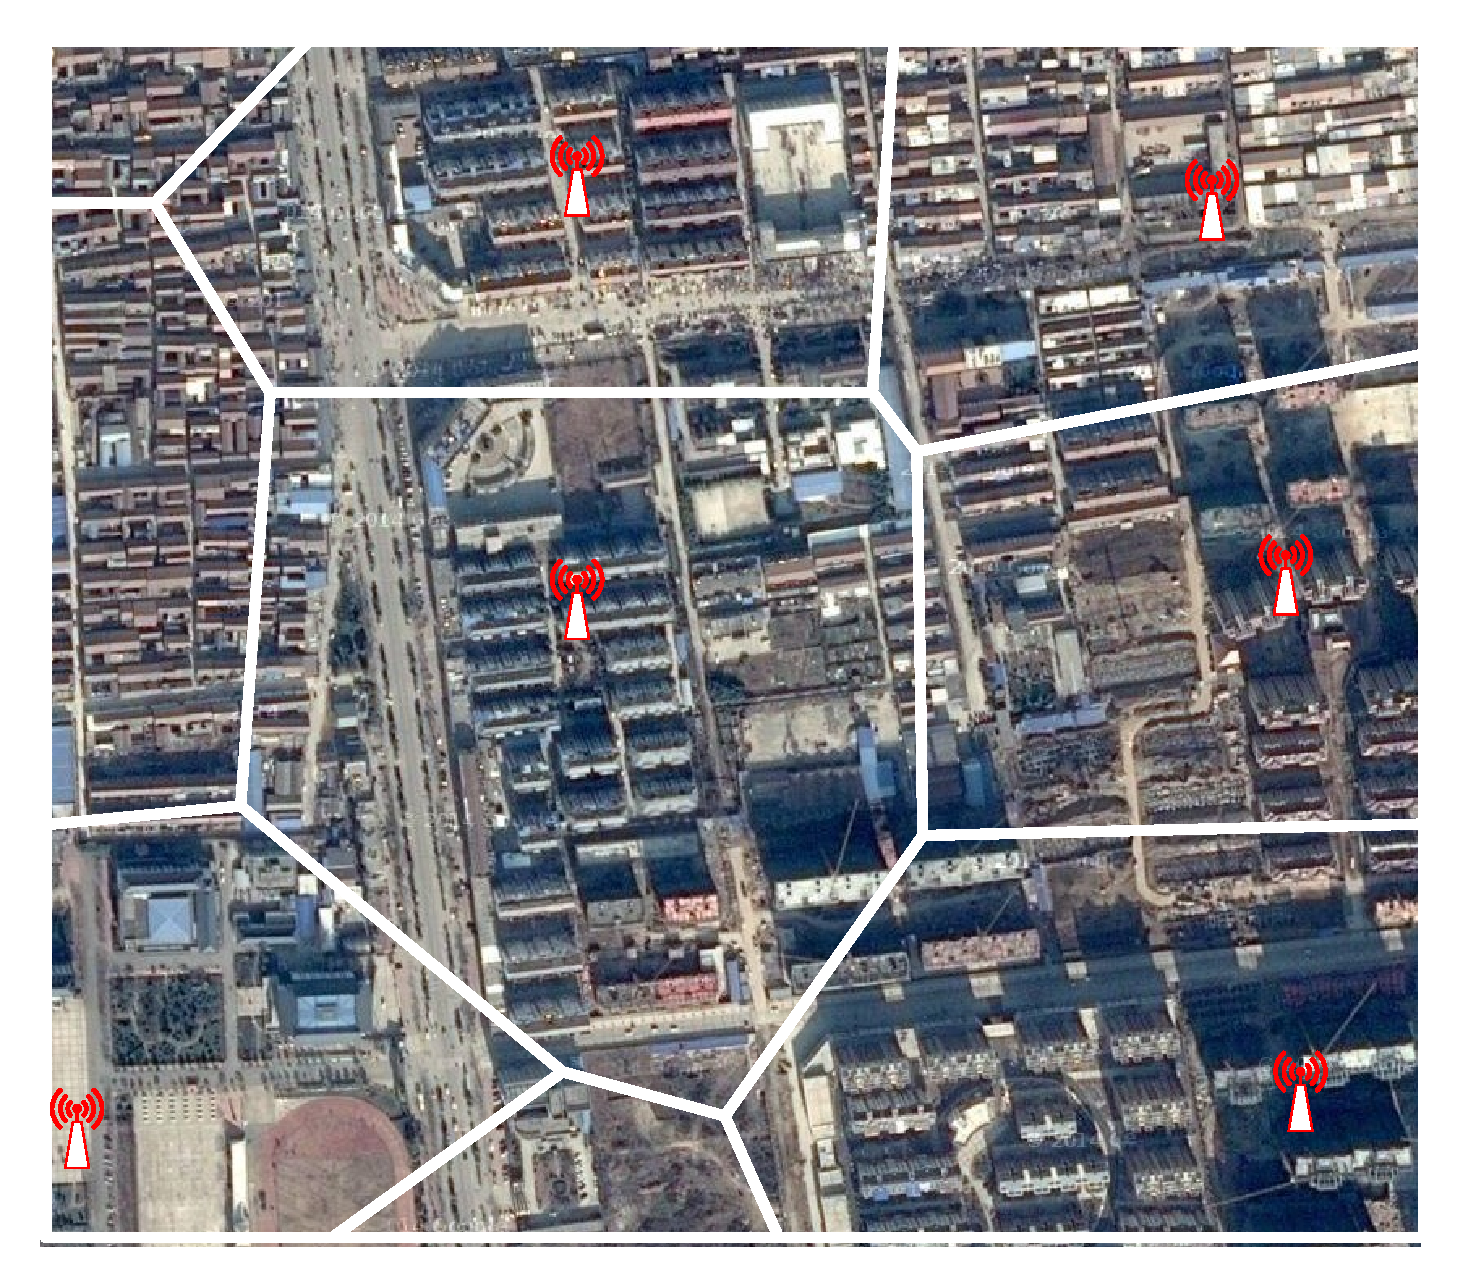
\includegraphics[width=\linewidth]{./figures/voronoi_illustrate.pdf}
    \caption{Voronoi diagram using Voronoi region to represent communication coverage of each tower}
		\label{fig:voronoi}
\end{figure}

To easily calculate the distance lower bound we first simplify the tower coverage model by assuming the cell phones only communicate with the nearest tower. With this assumption, we can use equirectangular projection to reduce the tower coverage map to a Voronoi diagram with each tower's location as Voronoi points. Fig.~\ref{fig:voronoi} shows an example of the Voronoi diagram containing five towers. Each region in the Voronoi diagram represents the coverage area of the related tower. Boundaries of regions in Voronoi diagram represent the overlapped boundaries area of towers. Then the shortest distance required to travel from one boundary to another boundary can be simplified as the shortest distance of two Voronoi boundaries. 

If we have an estimated distance that is much larger than the distance lower bound, then it is likely that the two boundaries could have paths of various distances. So using one distance estimation to represent the distance of all possible path may not be accurate. On the contrary, if the estimated distance is very close to the distance lower bound, then the estimated distance should be able to represent the distance of most paths between two boundaries. The distance lower bounds can also help to eliminate the problem of false passing boundary events. Since the user keeps passing the same boundary, the distance lower bound for such scenarios is always $0$. 

For the distance estimates, other than estimating with the trajectory that has the maximum likelihood with visited tower sequence, which require the knowledge of underlying road network. We use a very simple scheme that only require tower coordinates to estimate distances of two boundaries. Suppose one PBE is from $l_i$ to $l_j$, and the other one is from tower $l_j$ to $l_k$. We first calculate straight line distance $d(l_i,l_j)$ and $d(l_j,l_k)$ by using tower's coordinates. Since the boundaries are perpendicular bisector of straight lines connecting towers, then the travel distance can be estimated by $\frac{d(l_i,l_j) + d(l_j,l_k)}{2}$. 

\begin{figure}[h]
    \centering
    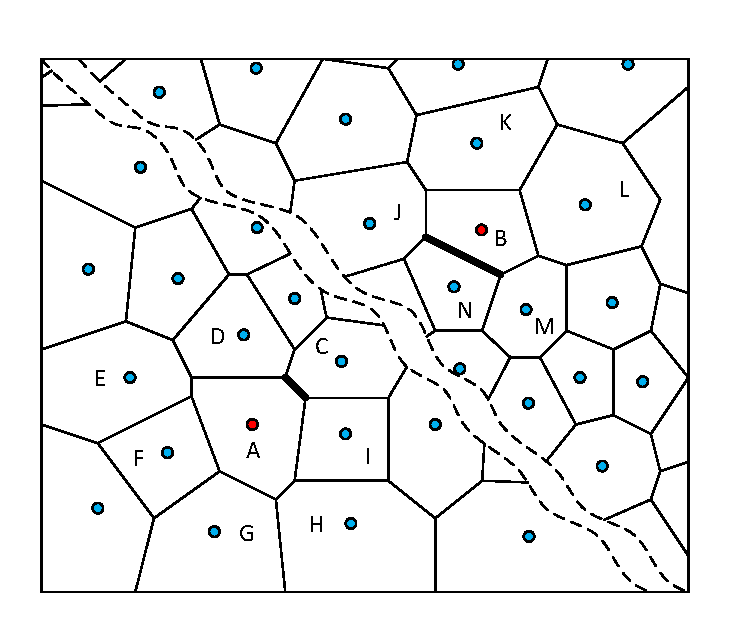
\includegraphics[width=\linewidth]{./figures/virtual_boundary.pdf}
    \caption{Deal with virtual boundaries}
		\label{fig:virtual}
\end{figure}

Remember that a real boundary means overlapped communication coverage areas while a virtual boundary means there is no overlap between the communication coverage areas of the towers. Different from real boundaries that are treated as a line which does not have distance for itself in distance estimations, virtual boundaries actually have distance estimates due to the fact that user have passed the coverage area of several towers. But we do not have the information of which boundaries does the user pass through for a virtual boundary. So to calculate the distance of a virtual boundary that connect tower $l_i$ to $l_j$, we use the shortest distance of all possible boundary pairs of $l_i$ and $l_j$. For example in fig.~\ref{fig:virtual}, suppose two consecutive records $r_i$ is the user's last record in tower A, $r_j$ is the user's first record in tower B. Since tower A and tower B does not share a boundary, so the related PBE has a virtual boundary. To calculate the distance, we calculate the distance from each boundary of tower A to each boundary of tower B, and use the distance of the shortest distance of all boundary pairs. In this example, the distance between boundary (A, C) and boundary (B, N) is used.

\subsection{Extract user speed}

\subsubsection{speed estimation}

To infer user's speed during each aggregate record, the PBEs with real boundaries are used as reference points since they have better location accuracy as mentioned above. For aggregate records that have PBEs with virtual boundaries, we merge them with adjacent aggregate records if there is any. The distance estimates and distance lower bound of the merged record is the sum of distance estimates and distance lower bound of both records and the virtual boundary between them. Note that when we sum up distance lower bounds, the result is still the minimum distance required to reach one real boundary from the other one that passing through virtual boundaries in between following visited tower sequence in the trace. We denote real boundaries by $b$. Suppose the two PBEs are $P_{i,j}$ with real boundary $b{i,j}$ and $P_{k,l}$ with real boundary $b_{k,l}$. Then the distance estimate and the distance lower bound between them are denoted by $d_{est}(b_{i,j}, b_{k,l})$ and $d_{lb}(b_{i,j}, b_{k,l})$.

For the duration between two reference points (PBEs with real boundaries), we can simply use the time difference of the PBEs. Note that for each PBE, the time related to it is not a time point but a time interval, We will have two durations, a tight duration which is the time difference of the first and last record belonging to the aggregate record between two reference points and a loose duration which is the time difference of two records that does not belong to the aggregate record between the reference points. For example, for two PBEs $P_{i,j}$ and $P_{k,l}$ with time interval $(t_i, t_j)$ and $(t_k, t_l)$ respectively. Suppose $P_{i,j}$ happens before $P_{k,l}$, then $t_i \leq t_j \leq t_k \leq t_l$. We denote the tight duration by $\Delta t_{tight} = t_k - t_j$ and loose duration by $\Delta t_{loose} = t_l - t_i$. So the estimated duration of the aggregate record between $P_{i,j}$ and $P{k,l}$ can be calculated by $frac{\Delta t_{tight} + \Delta t_{loose}}{2}$, we denote it by $\Delta t_{est}$.

Large differences between $d_{est}$ and $d_{lb}$ or between $\Delta t_{tight}$ and $\Delta t_{loose}$ indicate inaccuracy in distance estimate or duration estimate respectively. So before we estimate the speed, we set up a set of criterion to filter out these records with possible inaccurate estimates:

\begin{equation}
  d_{ratio} = \frac{d_{lb}}{d_{est}}
\end{equation}
\begin{equation}
	\Delta t_{ratio} = \frac{\Delta t_{tight}}{\Delta t_{loose}}
\end{equation}

By setting a threshold for both criterion, we can filter out speed estimates that are not accurate enough. Although we can filter out more possible inaccurate speed estimates with very strict threshold in both criterion, we may end up with limited number of records that have qualified speed estimates.

For aggregate records which meet both criterion, we calculate their speed estimates $s$ as following:

\begin{equation}
  s_{est} = \frac{d_{est}}{\Delta t_{est}} 
\end{equation}

\subsubsection{speed compensation}

Due to the false passing boundary event mentioned in left part of fig.~\ref{fig:illustrate_cases}, a large number of records will have a distance lower bound with a value of $0$. And they will eventually been filtered by out distance criterion so that they will not receive any speed estimates. Since these aggregate records usually have very short duration due to the nature of how they are generated. One way to estimate the speed for such records are based on the assumption that a user's speed does not change dramatically in a very short time period. So for a aggregate record with false passing boundary event, if there is an aggregate record that are happened very close to them and have a qualified speed estimates, then we will use its speed estimates as the speed estimates for the record with false passing boundary event.
